
%---------------------------- Beginning of preamble


%-------- document class
% comment this line if you want to print the presentation and uncomment the next one
\documentclass[9pt, hide notes, hyperref={pdfpagelabels=false}]{beamer} 
% comment this line if you want to show the presentation and uncomment the previous one
%\documentclass[9pt, handout, hyperref={pdfpagelabels=false}, allowframebreaks]{beamer} 


%-------- general layout
\mode<presentation>
{
  
  	%---- themes
  	\usetheme{Antibes}
  	%\usetheme{Singapore}
  	%\usetheme{Warsaw}
	
	%nice theme for math fonts
	\usefonttheme{professionalfonts}

	%color theme
	\usecolortheme{lily}

	  %for math characters
  	\usefonttheme[onlylarge]{structuresmallcapsserif}
	\usefonttheme[onlysmall]{structurebold}
	
	%remove navigation symbols
	\setbeamertemplate{navigation symbols}{}

	%dark blue for normal text
	\definecolor{MyDarkBlue}{rgb}{0.0235,0.1569,0.4745}
	\setbeamercolor{normal text}{fg = MyDarkBlue}
	
	%white for background text color
	\setbeamercolor{structure}{bg = white}
		
	%---- headline
	% black and white for headline and footline
	\setbeamercolor{section in head/foot}{bg = white, fg=black}
	\setbeamercolor{subsection in head/foot}{bg = white, fg=black}
	\setbeamercolor{title in head/foot}{bg = white, fg=black}	
	
	%What do you want in your header? by default, there is the current subsection
	
	%if you want to insert a complete navigation	
		\setbeamertemplate{headline}
		{%--
			\begin{beamercolorbox}{section in head/foot}
				\vskip2pt\insertnavigation{\paperwidth}\vskip2pt
			\end{beamercolorbox}
		}%--
	
	%---- footline	
	%add frame number and logo
	\setbeamertemplate{footline}
	{%--
	   %you can adjust the left and right white space with leftskip and rightskip
	\begin{beamercolorbox}[ht=2.5ex,dp=1.125ex,
	    leftskip=.15cm,rightskip=.15cm plus1fil]{title in head/foot}
	     \insertframenumber/\inserttotalframenumber
	     \hspace{0.5cm}	%you can use different horizontal spacing!
	     \insertshortdate
	     \hfill
	\end{beamercolorbox}
  	}%--
  
	%% No footline on title slide
	\defbeamertemplate{footline}{title slide}{%
	\relax
	}
	
		
	%---- misc
  %\setbeamercovered{transparent}
  % or whatever (possibly just delete it)
  

}


%-------- packages import
%language
\usepackage[english]{babel}
%\usepackage[frenchb]{babel}
% or whatever

%UNIX accent encoding
\usepackage[latin1]{inputenc}

\usepackage{wrapfig}

\usepackage{times}
\usepackage[T1]{fontenc}
% Or whatever. Note that the encoding and the font should match. If T1
% does not look nice, try deleting the line with the fontenc.

%math symbols
\usepackage{amsmath,amsfonts,amssymb,latexsym,qsymbols}

\usepackage{multirow}


% les macros
\newcommand\HRule{\noindent\rule{\linewidth}{1pt}}
\newcommand{\II}{\mbox{\large 1\hskip -0,353em 1}}
\newcommand{\abs}[1]{\lvert#1\rvert}
\newcommand{\norm}[1]{\lVert#1\rVert}
\newcommand{\ligne}{\rule[2mm]{.3\textwidth}{0,5mm}\\}
\newcommand{\pkg}{\textbf}
\newcommand{\sigle}{\textsc}
\newcommand{\code}{\texttt}
\newcommand{\soft}{\textsf}
\newcommand{\myskip}{\vspace{\parskip}}
\newcommand{\txtm}[1]{\textrm{~~#1~~}}
\newcommand{\expo}{\textsuperscript}
\newcommand{\ind}{1\!\!1}
\newcommand{\mat}[1]{\mathbf{#1}}
\newcommand{\blank}{ \clearpage{\pagestyle{empty}\cleardoublepage} }
\newcommand{\card}{\textrm{Card}}
\newcommand{\clg}{\textrm{clg}}
\newcommand{\mbbR}{\mathbb R}
\newcommand{\Var}{\textrm{Var}}
\newcommand{\Jac}{\textrm{Jac~}}

%-------- fill information used for frames

%---- title
\title[Prob Dist Fit] % (optional, use only with long paper titles)
{A Unified Approach for Probability Distribution Fitting with \pkg{fitdistrplus}}

%---- author
\author % (optional, use only with lots of authors)
{M-L.~Delignette-Muller\inst{1}, C.~Dutang\inst{2,3}}
% Give the names in the same order as the appear in the paper.
% Use the \inst{?} command only if the authors have different affiliation.

%---- affiliation to a particular organisation, institution or company
\institute % (optional, but mostly needed)
{
  \inst{1}%--
  VetAgro Sud Campus V�t�rinaire - Lyon
  \inst{2}%--
  ISFA - Lyon,
  \inst{3}%--
  AXA GRM - Paris,
}
% Use the \inst command only if there are several affiliations.
% Keep it simple, no one is interested in your street address.


%---- date
\date[12/08/2011] % (optional, should be abbreviation of conference name)
{
\includegraphics[height=1cm]{img/useR-middle2} \Huge{2011}}
% Either use conference name or its abbreviation.
% Not really informative to the audience, more for people (including
% yourself) who are reading the slides online

%---- subject
\subject{Probability distribution fitting methods}
% This is only inserted into the PDF information catalog. Can be left
% out. 

%---- To plot table of contents at the begin of...
% Delete this, if you do NOT want the table of contents to pop up at
% the beginning of each section:

%\AtBeginSection[]
%{%--
%  \begin{frame}%<beamer>
%    \frametitle{Outline}
%    \tableofcontents[current,currentsection]
%  \end{frame}
%}%--


\newcommand{\red}[1]{\textcolor{red}{#1}}

\newcommand{\black}[1]{\textcolor{black}{#1}}

%---------------------------- End of preamble

%---------------------------- Beginning of presentation body
\begin{document}


%---- title page
\begin{frame}
  \titlepage
  \vspace{-.5cm}
  \centering
  
  
\end{frame}

%---------------------------------------------------------------------------------------------------------
\section*{Introduction}


%---- title outline/agenda
\begin{frame}
  \frametitle{Outline}
  \setcounter{tocdepth}{1}
  \tableofcontents
  
\end{frame}



%---------------------------------------------------------------------------------------------------------
\section[MLE]{Maximum likelihood estimation}
\subsection{MLE}

\begin{frame}[fragile]{Maximum likelihood estimation - brief reminder}
Assuming a  sample $(X_i)_{1\leq i \leq n} \stackrel{i.i.d.}{\sim} X$, the likelihood
$$
\mathcal L(\theta, x_1, \dots, x_n ) %= \prod_{i=1}^n f_{X_i}(x_i, \theta ) 
= \prod_{i=1}^n f_X(x_i, \theta ),
$$
where $f_{X}$ is the generic mass probability/density function.


The MLE estimator $\theta_{\text{MLE}}$ maximizes the likelihood %$\mathcal L$ or $\log \mathcal L$.
$$
\theta_{\text{MLE}} = \underset{\theta \in \Theta}{\arg\max}~ \mathcal L(\theta, x_1, \dots, x_n ) .
$$

Example %> library(fitdistrplus)
%> x1 <- c(6.4,13.3,4.1,1.3,14.1,10.6,9.9,9.6,15.3,22.1,13.4, ...
%+ 13.2,8.4,6.3,8.9,5.2,10.9,14.4)
%$optim.function
%[1] "optim"
\begin{scriptsize}
\begin{verbatim}
> (f1 <- mledist(x1,"norm"))
$estimate
     mean        sd 
10.411111  4.747033 
$convergence
[1] 0
$loglik
[1] -53.57625
$hessian
          mean       sd
mean 0.7987816 0.000000
sd   0.0000000 1.597564
\end{verbatim}
\end{scriptsize}


\end{frame}

\begin{frame}[fragile]{Function \code{mledist} with non \soft{R}-base distributions}

\begin{scriptsize}
\begin{verbatim}
> dgumbel<-function(x,a,b) 1/b*exp((a-x)/b)*exp(-exp((a-x)/b)) 
> (f2 <- mledist(x1,"gumbel",start=list(a=10,b=5)))
$estimate
       a        b 
8.094333 4.375401 
$convergence
[1] 0
$loglik
[1] -54.09525
$hessian
           a          b
a  0.9400408 -0.4418806
b -0.4418806  1.9124424
\end{verbatim}
\end{scriptsize}

\begin{figure}
\begin{center}
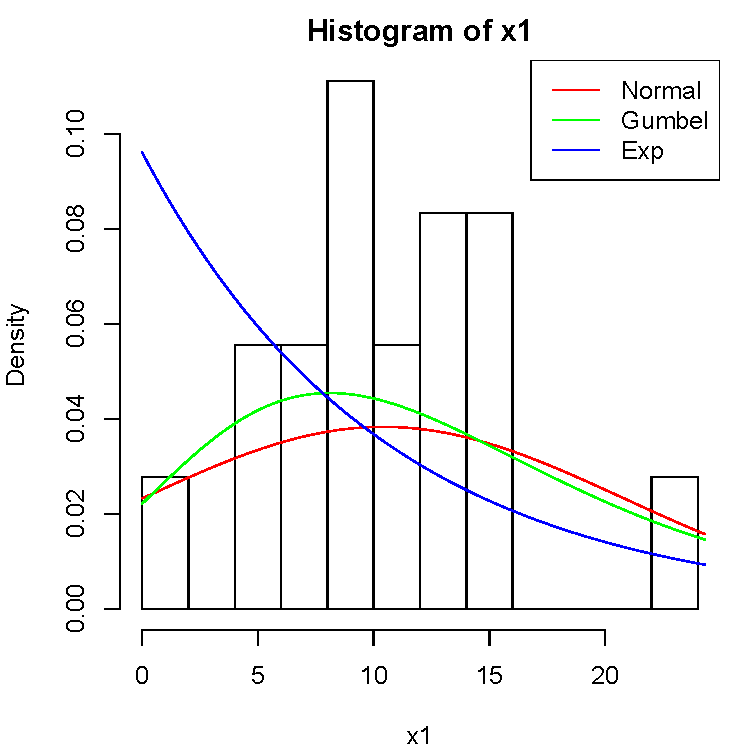
\includegraphics[height=0.5\textheight]{img/x1_hist} 
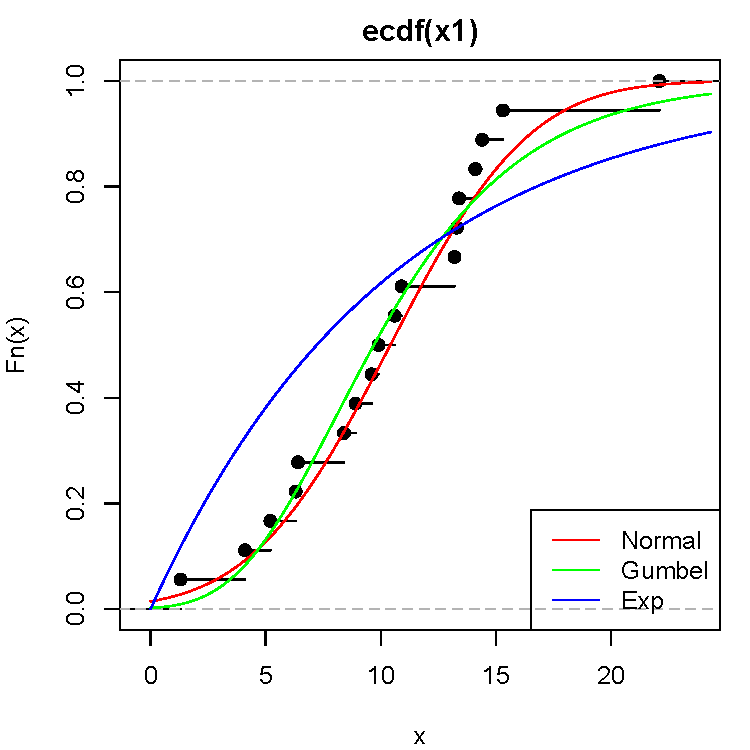
\includegraphics[height=0.5\textheight]{img/x1_ecdf} 
\end{center}
\end{figure}



\end{frame}

\begin{frame}[fragile]{Optional arguments of \code{mledist}}


\begin{columns}

\begin{column}{0.4\textwidth}

Fixed arguments
\begin{scriptsize}
\begin{verbatim}
> (f4 <- mledist(x1, "gumbel", 
start=list(b=5), fix.arg=list(a=7) ))
$estimate
       b 
4.248811 

$convergence
[1] 0

$loglik
[1] -54.60187

$hessian
         b
b 1.710569

$optim.function
[1] "optim"

> f2
$estimate
       a        b 
8.094333 4.375401 
\end{verbatim}
\end{scriptsize}
\end{column}

\begin{column}{0.6\textwidth}

Custom optimization
\begin{scriptsize}
\begin{verbatim}
> fit1 <- mledist(x1, "gamma")
> 
> fit1bis <- mledist(x1, "gamma", optim.method="BFGS")
> 
> #wrap genoud function 
> mygenoud <- function(fn, par, ...) 
+ {
+ 	require(rgenoud)
+	res <- genoud(fn, starting.values=par, ...)        
+ 	standardres <- c(res, convergence=0)
+ 	return(standardres)
+ }
> 
> #custom optimization call
> fit2 <- mledist(x1, "gamma", custom.optim=mygenoud, 
+ 	nvars=2, Domains=cbind(c(0,0), c(10, 10)), 
+ 	boundary.enforcement=1, print.level=0, hessian=TRUE)
>
> cbind(NelderMead=fit1$estimate, BFGS=fit1bis$estimate, 
+ Genoud=fit2$estimate)
      NelderMead      BFGS    Genoud
shape  3.5747819 3.5768812 3.5742223
rate   0.3433516 0.3435683 0.3433094
\end{verbatim}
\end{scriptsize}
\end{column}

\end{columns}

\end{frame}


%---------------------------------------------------------------------------------------------------------
\section[MME]{Moment matching estimation}
\subsection{MME}

\begin{frame}[fragile]{Moment matching estimation}
It consists in equating the theoretical moments and the empirical moments
$$
E\left[X^k; \theta \right]  = \frac{1}{n} \sum_{i=1}^n X_i^k, \txtm{for} k=1, \dots, p.
$$
with $\theta \in \mathbb R^p$.

$\theta_{\text{MME}}$ can be computed in two ways, either by closed formulas (e.g. exponential distribution) or by square residual numeric minimization.

Example with closed formulas
\begin{columns}

\begin{column}{0.5\textwidth}
\begin{scriptsize}
\begin{verbatim}
> (g1 <- mmedist(x1, "norm"))
$estimate
     mean        sd 
10.411111  4.747033 

$convergence
[1] 0

$order
[1] 1 2

$memp
NULL
\end{verbatim}
\end{scriptsize}
\end{column}

\begin{column}{0.5\textwidth}
\begin{scriptsize}
\begin{verbatim}
$loglik
[1] -53.57625

$method
[1] "closed formula"

> cbind(MLE=f1$estimate, MME=g1$estimate)
           MLE       MME
mean 10.411111 10.411111
sd    4.747033  4.747033
\end{verbatim}
\end{scriptsize}
\end{column}

\end{columns}

\end{frame}

\begin{frame}[fragile]{\code{mmedist} - Example with numerical optimization}



\begin{columns}

\begin{column}{0.5\textwidth}


\begin{scriptsize}
\begin{verbatim}
> #empirical raw moment
> memp <- function(x, order)
+ 	ifelse(order == 1, mean(x), 
+	sum(x^order)/length(x))
> 
> #euler constant
> euler <- 0.5772156649
> 
> #theoretical raw moment
> mgumbel <- function(order, a, b)
+ {
+ 	mean <- a + b*euler
+ 	if(order == 1)
+ 		return(mean)
+ 	else
+ 		return(mean^2 + pi^2*b^2/6)
+ }
> 
> g2 <- mmedist(x1, "gumbel", order=c(1, 2), 
+	memp="memp", start=c(10, 5))
> 
> cbind(MLE=f2$estimate, MLEfix=c(8, 
+	f4$estimate[1]), MME=g2$estimate)
       MLE   MLEfix      MME
a 8.094333 8.000000 8.260669
b 4.375401 4.248811 3.713298

\end{verbatim}
\end{scriptsize}
\end{column}

\begin{column}{0.5\textwidth}

\begin{figure}
\begin{center}
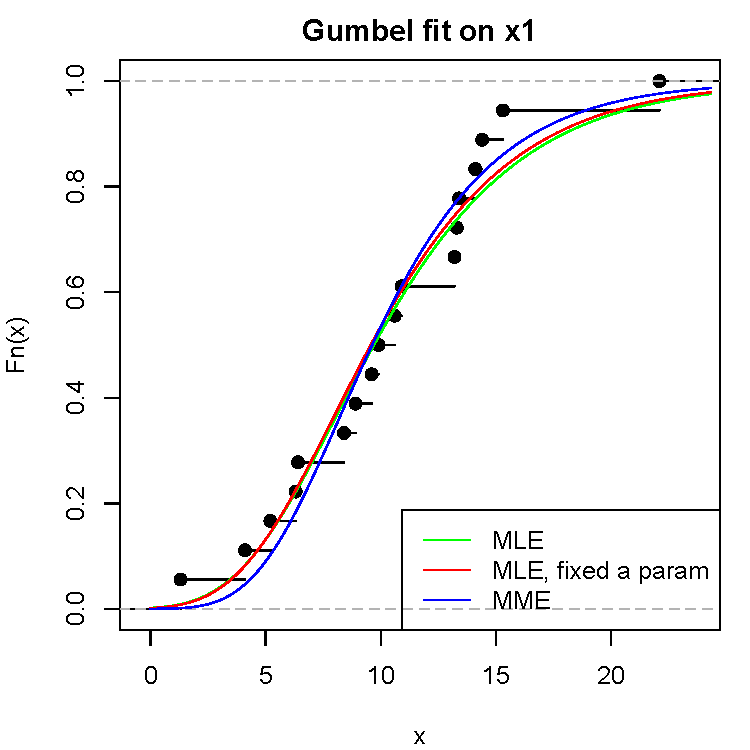
\includegraphics[height=0.72\textheight]{img/x1_mleVSmme} 
\end{center}
\end{figure}


%\begin{scriptsize}
%\begin{verbatim}

%\end{verbatim}
%\end{scriptsize}

\end{column}

\end{columns}



\end{frame}


%---------------------------------------------------------------------------------------------------------
\section[QME]{Quantile matching estimation}
\subsection{QME}

\begin{frame}[fragile]{Quantile matching estimation}
It consists in equating the theoretical quantiles and the empirical quantiles
$$
q_{n, p_k} = F_X^{-1}(p_k), \txtm{for} k=1,\dots, p
$$
where $q_{n, p_k}$ is the empirical quantile and $F_X^{-1}(p_k)$ the theoretical one. $p_k$ are given probabilities on which $\theta_{\text{QME}}$ is computed numerically.

Example with normal distribution

\begin{columns}

\begin{column}{0.5\textwidth}
\begin{scriptsize}
\begin{verbatim}
> (h1 <- qmedist(x1, "norm", prob=c(1/2, 2/3)))
$estimate
     mean        sd 
10.250030  6.926297 

$convergence
[1] 0

$value
[1] 2.722893e-09

$hessian
          mean        sd
mean 4.0000000 0.8614546
sd   0.8614546 0.3710520

\end{verbatim}
\end{scriptsize}
\end{column}

\begin{column}{0.5\textwidth}
\begin{scriptsize}
\begin{verbatim}

$probs
[1] 0.5000000 0.6666667

$optim.function
[1] "optim"

$loglik
[1] -55.60913

> h1bis <- qmedist(x1, "norm", prob=c(1/3, 2/3) )
>
> cbind(MLE=f1$estimate, MME=g1$estimate, 
+ QME1=h1$estimate, QME2=h1bis$estimate)
           MLE       MME      QME1      QME2
mean 10.411111 10.411111 10.250030 10.983327
sd    4.747033  4.747033  6.926297  5.223794
>
\end{verbatim}
\end{scriptsize}
\end{column}

\end{columns}


\end{frame}



\begin{frame}[fragile]{\code{qmedist} example}



\begin{columns}

\begin{column}{0.5\textwidth}


\begin{scriptsize}
\begin{verbatim}
> #empirical quantiles computed with 
> #the quantile() function
>
> #theoretical quantiles
> qgumbel <- function(p, a, b)
+ 	a - b*log(-log(p))
> 
> h2 <- qmedist(x1, "gumbel", 
+	prob=c(1/3, 2/3), start=list(a=10, b=5))
> h2bis <- qmedist(x1, "gumbel", 
+	prob=c(1/2, 3/4), start=list(a=10, b=5))
> 
> 
> cbind(MLE=f2$estimate, MME=g2$estimate, 
+ QME1=h2$estimate, QME2=h2bis$estimate)
       MLE      MME     QME1     QME2
a 8.094333 8.260669 9.157968 8.947923
b 4.375401 3.713298 4.514493 3.553285

\end{verbatim}
\end{scriptsize}
\end{column}

\begin{column}{0.5\textwidth}

\begin{figure}
\begin{center}
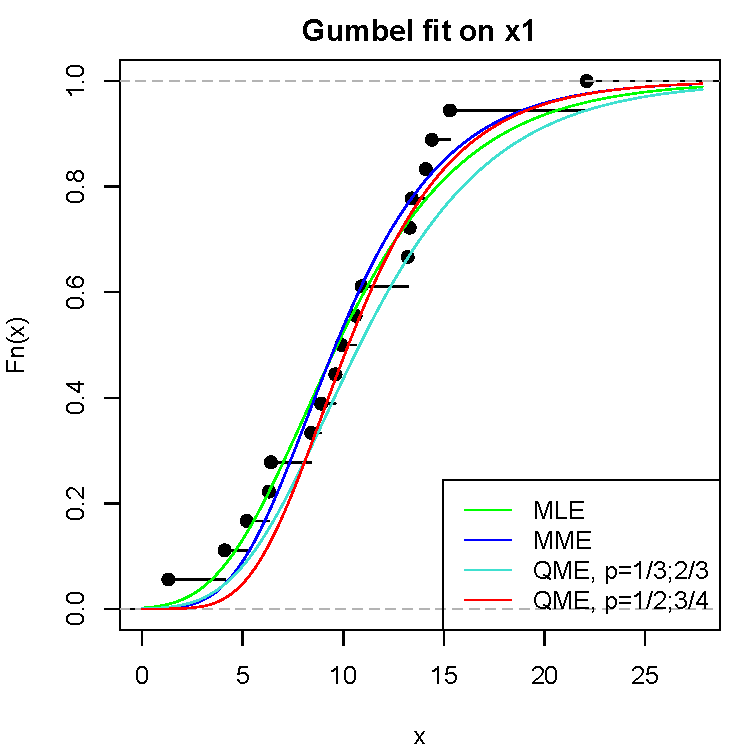
\includegraphics[height=0.72\textheight]{img/x1_mleVSmmeVSqme} 
\end{center}
\end{figure}

\end{column}

\end{columns}



\end{frame}



%---------------------------------------------------------------------------------------------------------
\section[MGE]{Maximum goodness-of-fit estimation}
\subsection{MGE}

\begin{frame}{Maximum goodness-of-fit estimation}
It consists in maximizing a goodness of fit statistics, or equivalently minimizing a distance. Generally, we use the following statistics
\begin{itemize}
\item Cram�r-von Mises: 
$$
\Delta^2_\text{CvM} = \int_{\mathbb R} \left( F_n(x) - F_X(x) \right)^2 dx,
$$
\item Kolmogorov Smirnov: 
$$
\Delta^2_\text{KS} = \underset{x}{ \sup}~ \left| F_n(x) - F_X(x) \right|,
$$
\item Anderson Darling:
$$
\Delta^2_\text{AD} = n \int_{\mathbb R} \frac{ \left( F_n(x) - F_X(x) \right)^2 }{ F_X(x)(1-F_X(x)) } dx,
$$
\end{itemize}
with $F_n$ the empirical cdf and $F_X$ the theoretical ones.

\end{frame}


\begin{frame}[fragile]{\code{mgedist} examples}



\begin{columns}

\begin{column}{0.5\textwidth}


\begin{scriptsize}
\begin{verbatim}
> i1_1 <- mgedist(x1, "norm", "CvM")
> i1_2 <- mgedist(x1, "norm", "KS")
> i1_3 <- mgedist(x1, "norm", "AD")
> 
> cbind(MLE=f1$estimate, CvM= i1_1$estimate, 
+ KS= i1_2$estimate, AD= i1_3$estimate)
           MLE      CvM        KS        AD
mean 10.411111 10.34687 10.643541 10.336154
sd    4.747033  4.64827  4.595217  4.763116
>
> 
> i2_1 <- mgedist(x1, "gumbel", "CvM", 
+	start=list(a=10, b=5))
> i2_2 <- mgedist(x1, "gumbel", "KS", 
+ start=list(a=10, b=5))
> i2_3 <- mgedist(x1, "gumbel", "AD", 
+ start=list(a=10, b=5))
> 
> cbind(MLE=f2$estimate, CvM= i2_1$estimate, 
+ KS= i2_2$estimate, AD= i2_3$estimate)
       MLE      CvM       KS       AD
a 8.094333 8.550061 8.736596 8.298506
b 4.375401 4.146123 3.916195 4.385616
> 
\end{verbatim}
\end{scriptsize}
\end{column}

\begin{column}{0.5\textwidth}

\begin{figure}
\begin{center}
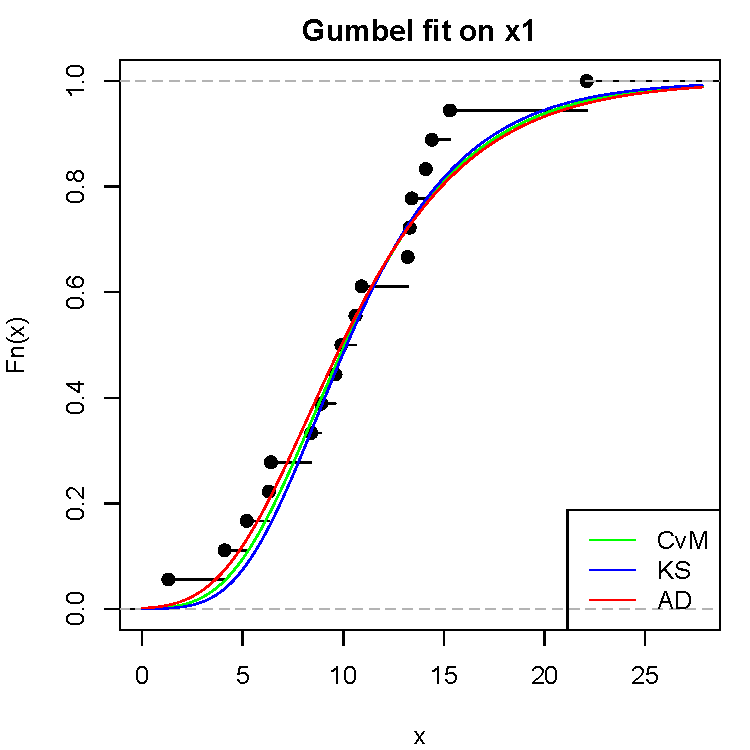
\includegraphics[height=0.72\textheight]{img/x1_mge} 
\end{center}
\end{figure}

\end{column}

\end{columns}



\end{frame}






%---------------------------------------------------------------------------------------------------------
\section[Censored]{Dealing with censored data}
\subsection{Censored}

\begin{frame}[fragile]{Censored data}

The $i$th obersvation $x_i$ is not known exactly, but rather somewhere on an interval $x_i \in ]l_i, u_i[$ with possible infinite bound. Non censored case is $l_i = u_i = x_i$.



\begin{columns}

\begin{column}{0.3\textwidth}


\begin{scriptsize}
\begin{verbatim}
> head(smokedfish, 10)
    left right
1     NA  0.04
2     NA  0.04
3   0.04 10.00
4   0.04 10.00
5     NA  1.00
6     NA  0.04
7   0.04 10.00
8   0.04 10.00
9     NA  0.04
10 15.00 15.00
> 
> plotdistcens(smokedfish)
> 
\end{verbatim}
\end{scriptsize}
\end{column}

\begin{column}{0.5\textwidth}

\begin{figure}
\begin{center}
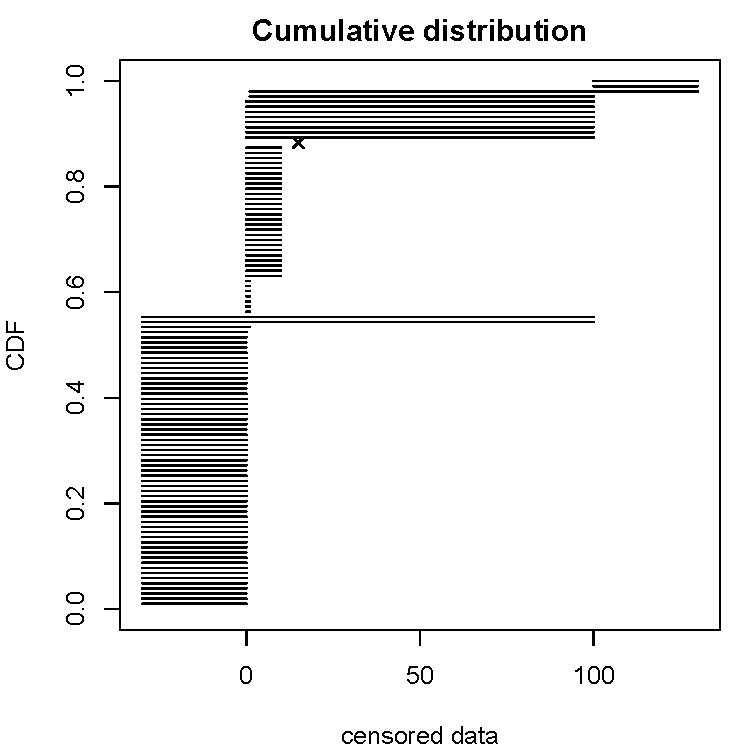
\includegraphics[height=0.72\textheight]{img/smokedfish_ecdf} 
\end{center}
\end{figure}

\end{column}

\end{columns}



\end{frame}

\begin{frame}{On the use of \code{mledistcens} }
Taking into account left and/or right censoring in the (log-)likelihood, maximum likelihood estimation can be carried out.

\begin{figure}
\begin{center}
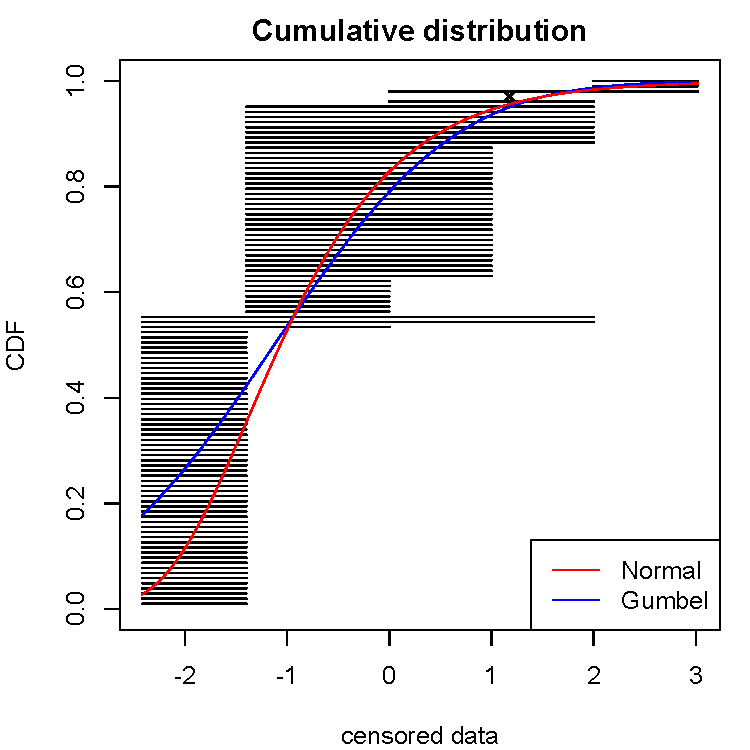
\includegraphics[height=0.72\textheight]{img/smokedfish_fit} 
\end{center}
\end{figure}


\end{frame}



%---------------------------------------------------------------------------------------------------------
\section*{Conclusion}

\begin{frame}{Conclusion (1/2)}

Functionalities of the \pkg{fitdistrplus} package
\begin{itemize}
\item MLE: Extends the \pkg{MASS} \code{fitdistr} function with fixed arguments, custom optimization algorithms, possible censoring,
\item MME: Provides a generic function to perform moment matching estimation with the raw or centered moments,
\item QME: Based on the \pkg{stats} \code{quantile} function, provides the quantile matching estimation,
\item MGE: Maximum goodness-of-fit is now available with the usual statistical distance and their variants.
\end{itemize}
So we can fit any probability distributions.

\bigskip

For specific probability distributions, please look at the task view \url{http://cran.r-project.org/web/views/Distributions.html}

\end{frame}



\begin{frame}[fragile]{Conclusion (2/2) - Unified approach with \code{fitdist} }

%Unified approach through the \code{fitdist} function and its \code{method} argument!



\begin{columns}

\begin{column}{0.45\textwidth}

\vspace{-1cm}
\begin{scriptsize}
\begin{verbatim}
> f0 <- fitdist(x1, "gamma", method="mle")
> 
> summary(f0)
Fitting of the distribution ' gamma ' 
by maximum likelihood 
Parameters : 
       estimate Std. Error
shape 3.5747819  1.1403248
rate  0.3433516  0.1175915

Loglikelihood:  -54.44954   
AIC:  112.8991   
BIC:  114.6798 
Correlation matrix:
          shape      rate
shape 1.0000000 0.9313999
rate  0.9313999 1.0000000
> 
> plot(f0, col="turquoise")
> 
> descdist(x1, boot=10, boot.col="turquoise")
summary statistics
------
min:  1.3   max:  22.1 
median:  10.25 
mean:  10.41111 
estimated sd:  4.884657 
estimated skewness:  0.3433588 
estimated kurtosis:  3.755991 
> 
\end{verbatim}
\end{scriptsize}
\end{column}

\begin{column}{0.55\textwidth}

\begin{figure}
\begin{center}
\vspace{-.65cm}
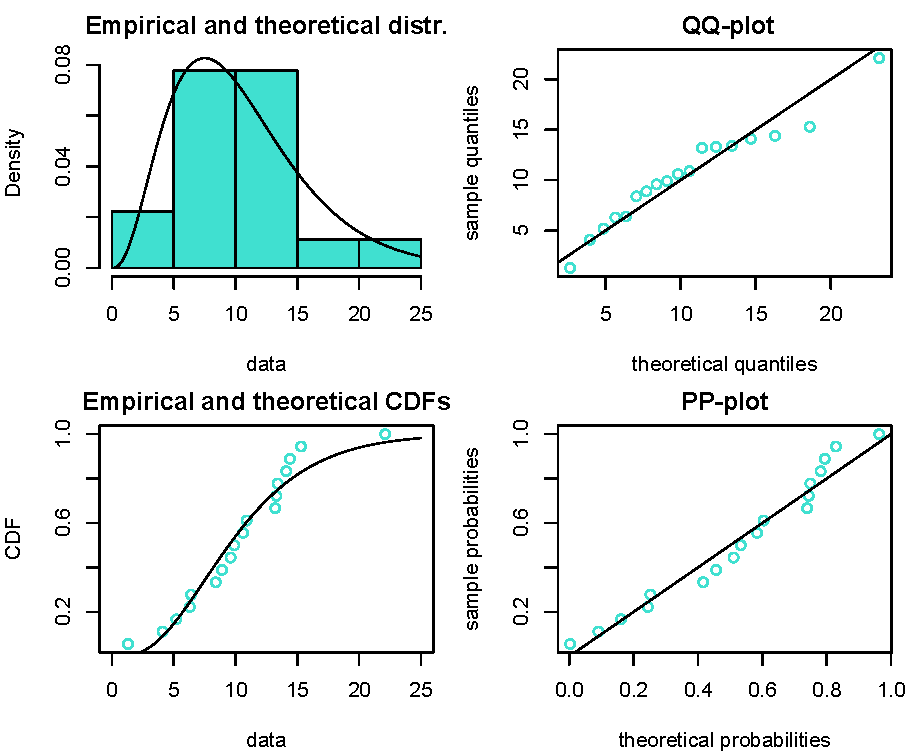
\includegraphics[height=0.45\textheight]{img/x1_graphcomp} 

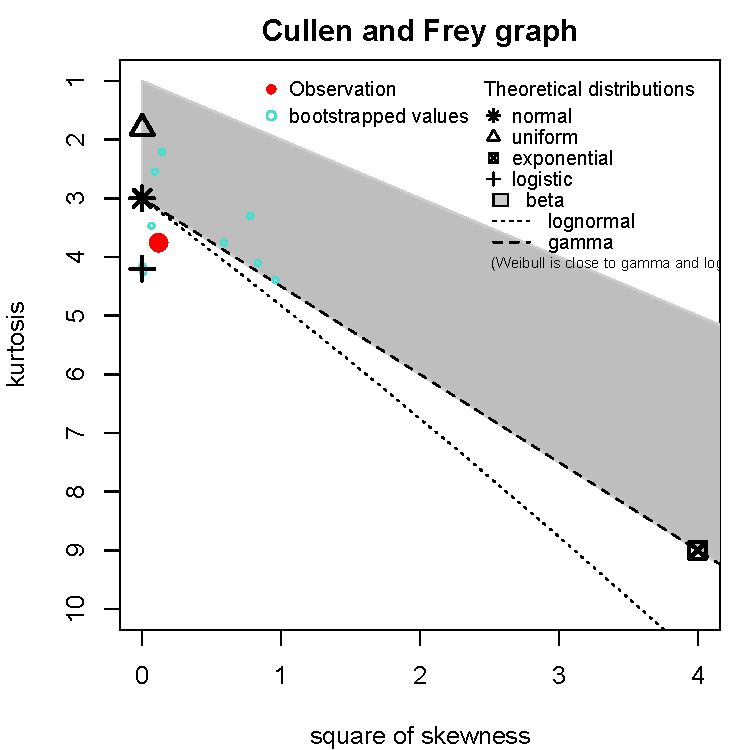
\includegraphics[height=0.49\textheight]{img/x1_cullenNfrey} 
\end{center}
\end{figure}

\end{column}

\end{columns}

\end{frame}






%---------------------------- End of presentation body
\end{document}


